\chapter{Análise de requisitos}

A análise dos requisitos dun produto software é unha parte fundamental do proceso de desenvolvemento, pois consiste definir de forma detallada o que debe facer o produto para satisfacer as necesidades e cumprir as expectativas do cliente.

O proceso de xestión de requisitos\cite{GPGR} consistirá en definir conxuntamente co cliente os distintos casos de uso do software. A partir dos casos de uso identificados extráense e documéntanse os requisitos, que se usarán como referencia para o desenvolvemento do sistema.

\section{Casos de uso}

Os casos de uso\cite{UseCase} describen as interaccións entre os actores é o sistema nunha linguaxe non técnica, centrándose en que fai sistema para o actor, entendendo por actor calquera entidade externa o sistema que lle demanda algunha funcionalidade.

Neste proxecto identifícase un único actor, que é o usuario xenérico da aplicación, pois nin existen distintos roles de usuarios nin outras entidades externas.

A continuación descríbense os casos de uso identificados en colaboración co cliente, e que se resumen graficamente na figura \ref{fig:uc}.

\uctable 	{CU.01}{Consultar as capacidades dun servidor SOS}
			{Consultar as capacidades dun servidor SOS para ver as ofertas que realiza e as propiedades dispoñibles nelas, e demais información do servizo.} %Propósito
			{É estendido polo \ref{uc:CU.02}} %Relacións
			{-} %Precondicións 
			{Visualízanse as capacidades do SOS nun formato amigable para o usuario.} %Postcondicións
			{O usuario introduce o enderezo do servidor SOS, ou selecciónao de entre os gardados. A aplicación descarga as capacidades do mesmo para amosalas en pantalla. 
			} %Escenario
			
\uctable 	{CU.02}{Obter observacións do servidor SOS}
			{Xerar unha capa vectorial cos datos das observacións rexistradas no SOS.} %Propósito
			{Estende o \ref{uc:CU.01}} %Relacións
			{Ter consultado as capacidades do servizo.} %Precondicións 
			{Capa vectorial coas observacións obtidas.} %Postcondicións
			{O usuario crea selecciona a través da interface gráfica a oferta e propiedades a consultar, así como outros filtros máis avanzados, por entidade de interese, sensor, período de tempo, filtros espaciais, etc. A aplicación descarga as observacións e xera unha capa vectorial en QGIS coa información procesada.
			} %Escenario

\uctable 	{CU.03}{Visualizar gráficas 2D}
			{Visualizar nunha gráfica en dúas dimensións a información das observacións a partir da capa xerada. Débese poder visualizar a evolución de unha propiedade o con respecto ó tempo, e tamén sería de utilidade en algúns caso poder enfrontar unha propiedade contra outra. } %Propósito
			{-} %Relacións
			{Ter xerada unha capa con datos de observacións.} %Precondicións 
			{Gráfico en dúas dimensións dos datos seleccionados.} %Postcondicións
			{Sobre a capa xerada o usuario seleccionará entidades de interese para poder visualizar nunha nova ventá un gráfico que represente o tempo no eixo X e a propiedade indicada no eixo Y. O usuario pode seleccionar outra propiedade para representar en cada un dos eixos.
			} %Escenario
			
\uctable 	{CU.04}{Visualizar mapas animados}
			{Facer visualizacións animadas dos datos da capa sobre o propio visor de mapas de QGIS.} %Propósito
			{-} %Relacións
			{Ter xerada unha capa con datos de observacións.} %Precondicións 
			{Visualización animada das observacións.} %Postcondicións
			{O usuario disporá duns controis de reprodución para as capas con datos de observacións de xeito que poda reproducir a evolución cronolóxica das observacións sobre o propio visor de mapas de QGIS. 
			} %Escenario

\begin{figure}[hbtp]
\centering
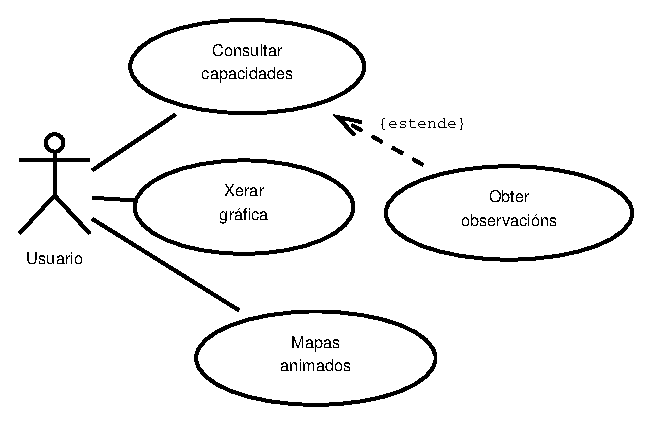
\includegraphics[scale=1]{images/uc.eps}
\caption{Diagrama de casos de uso}
\label{fig:uc} 
\end{figure}

\section{Catálogo de requisitos}
A partir dos casos de uso documentados realizase a extracción dos requisitos da aplicación. Estes requisitos son as características que debe presentar a aplicación, e definen o software desde o punto de vista do cliente. Dividimos os catálogo de requisitos en dúas partes, segundo a natureza dos mesmos:
\begin{description}
\item[Funcionais:] Son as características da aplicación para proporcionar a funcionalidade requirida.
\item[Non funcionais:] Non describen funcionalidades, se non que representan outras necesidades como seguridade, rendemento, usabilidade, ou restricións de plataforma, tecnolóxicas, e similares.
\end{description}

Clasificaremos os requisitos pola súa relevancia segundo o cadro \ref{tab:relevanciaReq}, que se terá en conta na planificación dos sprints.
\begin{table}
\begin{tabularx}{\textwidth}{lX} \toprule
	Relevancia & Descrición \\
	\midrule
	Esixido & Requisito que está directamente relacionado co cumprimento dos obxectivos do proxecto.\\
	Desexado & Requisito que mellora a calidade do proxecto, pero non está relacionado directamente cos obxectivos do mesmo.\\
	Opcional &  Requisito que non supón unha mellora substancial na calidade do proxecto, aínda que si resulta de utilidade.\\
	\bottomrule
\end{tabularx}
\caption{Niveis de relevancia dun requisito}
\label{tab:relevanciaReq}
\end{table}

\subsection{Requisitos funcionais}
Os requisitos funcionais definidos, verificados e revisados para o presente proxecto son os que seguen:

\reqtable 	{RF.01}{}
		  	{}%Descrición
			{}%Relevancia
			{}%Criterio de validación
			
\reqtable 	{RF.02}{}
		  	{}%Descrición
			{}%Relevancia
			{}%Criterio de validación
			
\reqtable 	{RF.03}{}
		  	{}%Descrición
			{}%Relevancia
			{}%Criterio de validación
			
\reqtable 	{RF.04}{}
		  	{}%Descrición
			{}%Relevancia
			{}%Criterio de validación

\subsection{Requisitos non funcionais}
Os requisitos non funcionais definidos, verificados e revisados para o presente proxecto son os que seguen:

\reqtable 	{RNF.01}{}
		  	{}%Descrición
			{}%Relevancia
			{}%Criterio de validación

\section{Matriz de trazabilidade}
A matriz de trazabilidade relaciona cada requisito co seu caso de uso de orixe. A matriz de trazabilidade para este proxecto é a representada no cadro \ref{tab:trazaRequisitos}.

\begin{table}[htbp]
\centering
\begin{tabular}{|l|c|c|c|c|}
\hline
 & CU.01 & CU.02 & CU.03 & CU.04 \\ \hline
RF.01 & $\bullet$ &  &  &  \\ \hline
RF.02 & $\bullet$ &  &  &  \\ \hline
RF.03 & $\bullet$ &  &  &  \\ \hline
RF.04 & $\bullet$ &  &  &  \\ \hline
RF.05 & $\bullet$ &  &  &  \\ \hline
RF.06 & $\bullet$ &  &  &  \\ \hline
RF.07 & $\bullet$ &  &  &  \\ \hline
RF.08 & $\bullet$ &  &  &  \\ \hline
RF.09 & $\bullet$ & $\bullet$ &  &  \\ \hline
RF.10 &  &  &  &  \\ \hline
RF.11 &  &  &  &  \\ \hline
RF.12 &  &  &  &  \\ \hline
RF.13 &  &  &  &  \\ \hline
RF.14 &  &  &  &  \\ \hline
RF.15 &  &  &  &  \\ \hline
RF.16 &  &  &  &  \\ \hline
RF.17 &  &  &  &  \\ \hline
RF.18 &  &  &  &  \\ \hline
RF.19 &  &  &  &  \\ \hline
RF.20 &  &  &  &  \\ \hline
\end{tabular}
\caption{Matriz de trazabilidade de requisitos}
\label{tab:trazaRequisitos}
\end{table}
